%The introduction is one of the most important pieces of your thesis.  Here is a place for you to introduce the problem(s) on which you have worked and place them in the larger context of your field.  You should aim to ensure that this section is completely understandable to virtually anyone - and certainly anyone with a sophomore-level grasp of physics.  Presumably this will include references to the literature.

%In addition to setting your work into context, a second good idea for your introduction is to give a short outline for what the rest of your thesis will discuss.  This is often done in the closing paragraph(s) of the introduction with sentences like ``In the following chapters \ldots " and ``Chapter 2 discusses \ldots"  Tremendous detail is not required in this outline, but rather just a brief road map for the rest of the document.

\section{Motivations}
Soft Condensed Matter Physics includes the study of colloids, liquid crystals, polymers, complex fluids, rubbers, foams, many biological materials, and - what we devote most of our time to studying in the Jensen lab - gels. From cosmetics to sticky notes, soft solids are ubiquitous in everyday life and are of growing interest due to their unique properties compared to traditional (hard) engineering materials. It is important to understand how such ubiquitous materials behave, especially when put under the strains of life. Accordingly, there 
 
 
 
\section{Historical Context}
\subsection{Development of Surface Tension}
Though few people may know the term, surface stress is a familiar concept in everyday phenomena: water droplets bead up into spheres, paperclips can float on water despite being made of dense iron, and water striders navigate the water's surface thanks to their hydrophobic legs. Each of these marvels is a result of \textbf{surface stress},$\Upsilon$, the  energetic cost per unit area to create new surface \cite{cammarata1994surface}. The water strider, for example, exerts a force on the water due to gravity. Because creating new surface costs energy, the water resists deformation, providing a restorative force that effectively balances the insect’s weight to keep it afloat. Likewise, water droplets bead up and liquid surfaces are smooth because $\Upsilon$ opposes surface stretching, acting to minimize the surface-to-volume ratio of the liquid \cite{gibbs1906scientific,GennesPierre-Gillesde2003Cawp} \todo[inline,color=green]{Consider returning here and adding after reading de Gennes}.

The energy associated with particles in the bulk is less than that of the particles at the surface. Molecules beneath the surface are attracted by the particles around them in every direction. In contrast, the particles at the surface are only attracted by the molecules directly adjacent to them. As a result of these less favorable interactions, they are in a state of higher energy compared to molecules in the bulk. The difference in energy between particles in the bulk compared to the surface is known as the \textbf{surface free energy}, $\gamma$, often written as just surface energy. Equivalently, $\gamma$ can also be defined as the reversible work per unit area to create new surface by cutting. This exposes new particles to the surface. When the surface of a fluid is stretched, however, new atoms or molecules arrive at the surface, maintaining the number of atoms per unit area as a constant value. Therefore, the surface energy is the same as the surface stress for a fluid and equal to a constant value. Because of this, $\gamma$ and $\Upsilon$ have are often referred to interchangeably as \textbf{surface tension}. While conceptually the energetics are similar in solid materials, the situation becomes more complicated for materials that cant flow.

\subsection{Surface Tension in Solids}
In metals, the origin of surface stress, on the atomic scale, derives from the crystalline structure. The epitaxial layer, or surface atoms, reside in a lower electron density and therefore a different equilibrium spacing than the bulk. The bulk atoms force the surface atoms to fit into the epitaxial overlayer of the crystalline substrate. As a result, the surface atoms are strained by the bulk, leaving the surface stressed by the underlying lattice \cite{cammarata1994surface}. 

\subsubsection{Strain Dependency of Surface Stress in Traditional Solids}
Although surface tension is most familiar in liquids, it is a property shared by solids as well.  In contrast to liquids, when a surface of a solid is elastically stretched, the number of atoms per unit area changes, such that generally $ \gamma \neq \Upsilon$ in solids \cite{cammarata1994surface}. The relationship between surface energy and surface stress can be derived through the use of the elastic deformation tensor $\epsilon_{ij}$, where $i,j=1,2$. We can then define $d\epsilon_{ij}$ to be an infinitesimal and elastic (reversible) strain as a result in a variation of the surface area, $A$. The surface stress tensor, $\Upsilon_{ij}$, is the work associated with the variation in the excess free energy of the surface due to strain, $\gamma A$. Thus, we can write, \[d(\gamma A) = A \Upsilon_{ij} d\epsilon_{ij}\] Expanding out the first term, $d(\gamma A) = \gamma dA + A d\gamma$. Utilizing symmetries, we can say that $dA = A \delta_{ij} d\epsilon_{ij}$, where $\delta_{ij}$ is the Kronecker delta. Making the substitution, we find \[\gamma dA + A d\gamma = \gamma A \delta_{ij} d\epsilon_{ij} + A d\gamma = A \Upsilon_{ij} d\epsilon_{ij}\] And thus,
\begin{equation}
\label{shuttleworth_eqn}
\Upsilon_{ij} = \delta_{ij}\gamma + \frac{\partial \gamma}{\partial \epsilon_{ij}} 
\end{equation}
This is known as the Shuttleworth Equation (\ref{shuttleworth_eqn}), and clearly shows that both $\gamma$ and $\Upsilon$ in solids are dependent on the strain state of the material.

Experimental measurements of surface stress have been around as early as the 1960, though measurements of strain-dependent surface stress have only been attempted much more recently and returned scant results \cite{mays1968surface,wasserman1970determination,hanneman1962elastic,martinez1990direct,schell1990mechanical}. Metals are an incredibly useful building tool due to their strength\footnote{Strength: the maximum force per unit area a material can withstand}, but their stiffness\footnote{Stiffness: the material's resistance to deformation via strain} also makes measuring properties as a function of strain severely limited, as most metals will fracture after a few percent strain.

For most solids, these surface effects go unnoticed in everyday life due to the overpowering effects of the bulk's elasticity compared to any surface energies. \todo[color=pink]{See Nat Comm 2017 ref 7-12}



\subsection{Surface Stress Effects in Soft Solids}
For solids of small enough size or soft enough composition, the surface energies can compete with or even dominate the effects of the bulk, resulting in strange and counterintuative physics. For example, the addition of finite, microscopic, liquid droplets in a soft solid actually stiffens the material \cite{style2015stiffening}, and stiffening micropillars are far stiffer than conventional physical theory predicts. \todo[color=pink]{Revise after reading papers}
\todo[inline,color=green]{Not toally sure what KEJ wants me to talk about. Would like ask in person.\\-Contact Lines zoom in\\-Liquid inclusions\\-Rayleigh Plateau\\-Instability\\-Rounding corners\\-adhsion (many?)}
Early observations of $ \Upsilon $ in soft solids came from consiering the wetting behavior of liquid droplets on soft solid surfaces.  The traditional Young-Dupre' picture of wetting is shown in Figure \ref{fig:three-phase}.
\begin{figure}[h!]
	\centering
	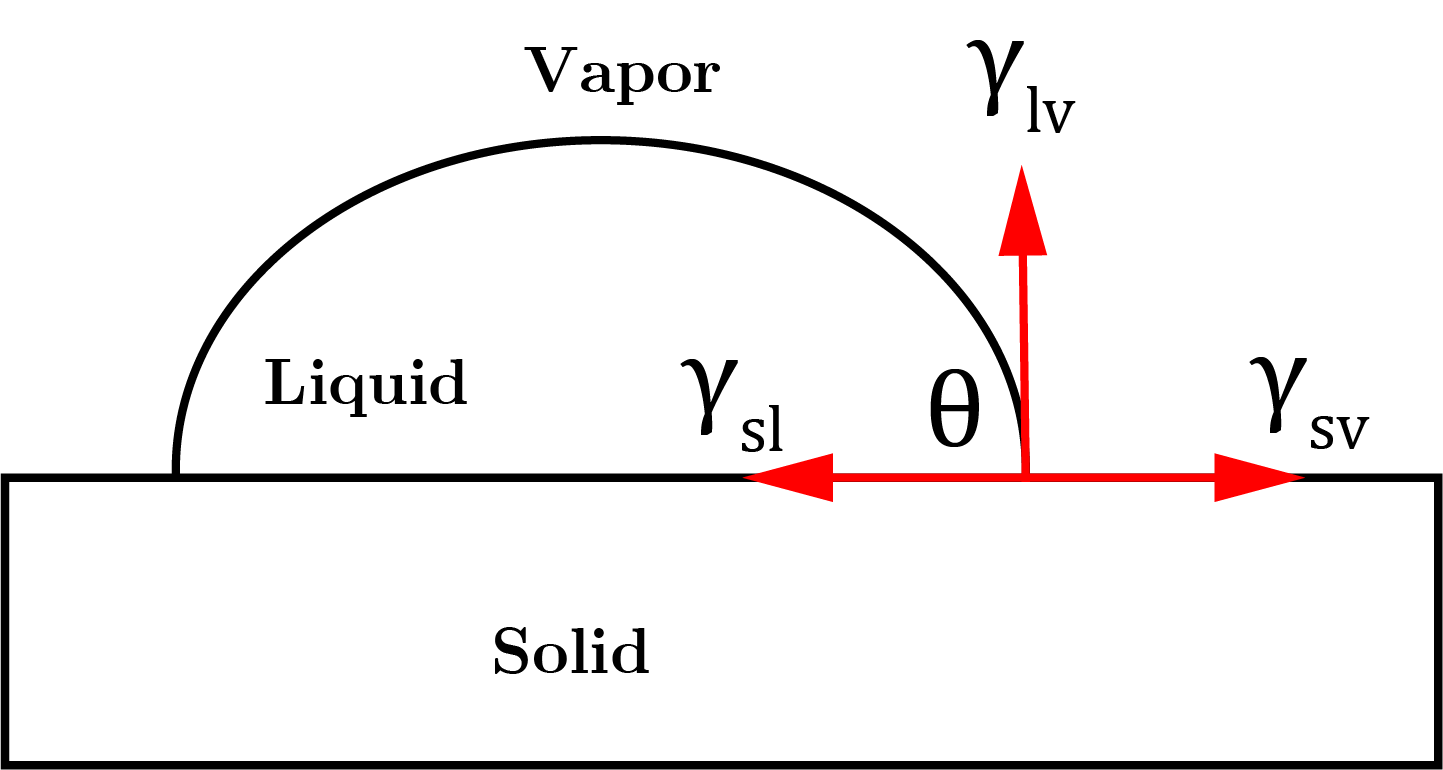
\includegraphics[width=.6\textwidth]{Chapters/Figures/phase_diagram.PNG}
	\caption[Three-Phase Diagram]{Classical Three-Phase Diagram]}
	\label{fig:three-phase} 
\end{figure}
\todo[inline, color=pink]{Include 3-phase zoom graphic}
This is clearly an unbalanced force diagram in vertical direction; the only vertical force component drawn is the liquid-vapor surface tension, $ \gamma_{lv} $. The normal force from $\gamma_{lv}$ must be balanced by the elastic substrate's resistance to deformation. Calculating this value, however, is still an open question. According to continuum elastic theory, the stress exerted by $\gamma_{lv}$ on the solid diverges at the contact line \cite{jerison2011deformation}. While Contact Mechanics dates back to the 18th century, seemingly simple problems like a liquid droplet on an elastic surface are still not yet well understood and provide challenging question when inspecting on a small enough scale.


\emph{The increased importance of surface stress in this regime leads to some material properties that are counter-intuitive to our everyday experiences. For example, soft solids can be stiffened with the inclusion of pockets of fluids below the elastocapillary length. In this regime, the surface tension dominates. Thus, the inclusion of a hole, while removing material affects the elastic stiffness, it also increases the surface area of the substrate. In this regime, this increase in surface area has a greater energetic cost, and thus leads to a solid of increased stiffness.}

Jerison et al. 2011 \cite{jerison2011deformation} found modeling the deformation of the elastic substrate due to a liquid droplet fit best with a model that incorporated both the finite thickness and surface tension of the substrate. This new model solved many issues with the previous best solution by Boussinesq: taking into account the finite thickness ensured that the deformations would go to zero far from the contact line, and the substrate's surface tension resolves the single stress singularity, eliminating the divergence of strain and vertical displacement at the origin. 
%Note to KEJ: I re-read Jerison 2011. I misread it the first time. In doing their calculations, they assumed the contact angle was close to $ 90\deg $, and they assumed $ \gamma_{sl}=\gamma_{sv} $...but their theory doesn't account for contact angles far from $ 90\deg $....which are the instances in which $ \gamma_{sl}\neq \gamma_{sv} $.


\subsection{Direct Measurement of Solid Surface Stresses}
Theoretical calculations for surface stress generally involve the taking the derivative of the predicted surface free energy with respect to strain. Various methods for metals involve calculating the electronic density, the kinetic energy, and the electrostatic exchange-correlation\footnote{Forgoing the independent electron approximation, the electronic exchange is a measure of deflection due to the presence of other electrons} \cite{GURTIN1978431}. 

Measuring the surface stresses even in soft solids has proved experimentally challenging over the years. \todo[color=yellow]{(Cite a few things here?)} A modern method of measuring the deformation of a soft, elastic solid imposed by the liquid droplet in Figure \ref{fig:three-phase} was introduced by Jerison in 2011 \cite{jerison2011deformation} and later utilized by Style \emph{et al.} in 2013 \cite{style2013universal}. They measured the 3-phase contact line geometry in figure \ref{fig:three-phase} without requiring any prior knowledge about the bulk elastic properties of the substrate material. 

\emph{While this technique is effective, it is limited in its applications due to material properties. The method only works for immiscible fluids such that the gel does not absorb the surface droplets. Furthermore, the fluid must also have a low volatility; otherwise, the droplet would begin to evaporate while waiting for the surface deformations to settle.}

\subsubsection{Puzzling Surface Stress Measurements in Gels}
In contrast to hard materials, it has been widely assumed that the surface stress in soft matter would be nearly strain-independent. Gels, for example, are comprised mainly of a fluid phase trapped between a solid mesh of polymers\footnote{For a more in depth explanation, see section \ref{section:polychem}}. Because the surface stress in liquids is constant and equal to the surface energy of the substance $(\Upsilon = \gamma)$, it was largely assumed that deforming a gel would not have a significant effect on the surface tension, given that the fluid could flow back to the stretched surface of the gel. 


In the following years, further tests of surface stress in soft solids (Table \ref{tab:upsilon_values}) were measured with wildly varying results. It began to become clear that the surface stress of soft solids was not simply that of the fluid phase, and there is more to the mystery. 
\begin{table}[h!]
	\centering
	\begin{tabular}{|l|l|l|l|}
		\hline
		\textbf{Silicone}       & \multicolumn{1}{c|}{\textbf{\begin{tabular}[c]{@{}c@{}}Young's Modulus \\ (kPa)\end{tabular}}} & \multicolumn{1}{c|}{\textbf{\begin{tabular}[c]{@{}c@{}}Measured $\Upsilon$ \\ (mN m$^{-1}$)\end{tabular}}} & \textbf{Reference} \\ \hline
		Sylgard 184             & 770                                                                       & 19                                & \cite{xu2016surface}                                                                       \\ \hline
		Gelest                  & 5.6                                                                       & 20                                                                                    &                    \cite{jensen2015wetting}\\ \hline
		Sylgard 184             & 2400                                                                      & 26                                                                                 &                 \cite{mondal2015estimation}   \\ \hline
			Dow Corning CY52-276A/B & 3                                                                         & 30                                                                                    &                 \cite{style2013universal}   \\ \hline
		Sylgard 184             & 18                                                                        & 30-70                                                                                 &                  \cite{jagota2012surface}\\ \hline
		Sylgard 184             & 1000                                                                      & 40-50                                                                                 &                 \cite{nadermann2013solid}   \\ \hline
		
	
		Dow Corning CY52-276A/B & 3                                                                         & 42-59                                                                                 &                  \cite{park2014visualization}  \\ \hline
	\end{tabular}
	\caption[Measured $\Upsilon$ Values]{A Collection of Previously Measured $\Upsilon$ Values}
	\label{tab:upsilon_values} 
\end{table}


While gels are technically classified as solids, they exhibit many properties that are more closely associated with liquids. Most notably, gels are comprised mainly of fluid (by weight). Their rigidity is the result of a three-dimensional network of crosslinked molecules which entrap large amounts of liquid throughout via capillary forces. The result is a solid whose stiffness is determined by the composition and temperature. Surface stress in soft solids is a topic of growing interest. Unlike in metals, elastocapillary physics plays a crucial role in determining the material's behavioral properties. In 2011, Jerison et. al \cite{jerison2011deformation} found that deformations of a silicone substrate due to a liquid droplet on the surface required the inclusion of surface tension. Furthermore, they determined that $\gamma_{sl}$ and $\gamma_{sv}$ must be dramatically different from one another, despite the previous assumption that the terms would be equal.

Soft solids provide a unique opportunity to measure strain-dependent surface stress. Despite being a solid, soft solids, such as gels, can easily be stretched elastically. In 2017, Xu, Jensen et. al published a paper \cite{xu2017direct} making the first direct measurement of strain-dependent surface stress in solids. Their measurements suggest a surprisingly strong linear relationship between surface-stress and strain, measuring that the surface stress of their PDMS substrate more than doubled at 20\% strain. \emph{To measure the surface stress of the material, the group utilized Jerison's 2011 method \cite{jerison2011deformation}. First, a glycerol or flurinaeted oil droplet is placed atop a soft, elastic silicone gel substrate. To measure surface deformations, the substrate is first coated with fluorescent beads, which can subsequently be measured using confocal microscopy. The located positions of the fluorescent beads outline the surface and allows for reconstruction of the surface deformations.} Additionally, their method of measurement is limited to a select combination of materials. We have developed a method for measuring strain dependent surface stress that is applicable to a wide variety of stretchable, soft materials.\todo[color=pink]{stretchable/ soft redundant?} To provide greater evidence of strain dependent surface stress, we made a separate measurement in PDMS as well as a variety of other soft materials using soft adhesion. In this thesis, I present the full background, methods, and underlying physics of the process.    


%Balancing, we find
%\[F_{vertical} = \gamma * \sin(\theta) = E * \delta,\]
%where $F_{vertical}$ is the force per unit length in the vertical direction, $\gamma$ is the surface tension of the liquid, E is the Young's modulus of a substrate, and $\delta$ is deformation of the substrate. Zooming


 



\subsubsection{Surface Tension and Contact with Soft Elastic Solids}
Over the last few years, there has been a significant amount of work regarding adhesion in soft solids. We want to take advantage of what is known about the role of surface stress in the contact mechanics of soft solids to directly measure the surface stress while varying the properties of the underlying substrate. In doing so, we will have created a new form of measuring strain-dependent surface stress, applicable to a broad array of stretchable materials. The contact angle based method used in the first direct measurement of $ \Upsilon(\epsilon) $ \cite{xu2017direct} is limited to a select combination of materials, as the liquid droplet must be immiscible and non-volatile. We hope to apply Jerison's 2011 technique to stretchable substrates in order to measure $ \Upsilon(\epsilon) $ for a wider variety of materials. The specifics of this technique are covered in the following chapter.

\section{Outline of the Thesis}
This thesis begins with a derivation of modern theory of contact mechanics for soft solids. With this in mind, we proceed to outline the experimental design and setup in chapter 2, followed with an example of data aquisition and image analysis in chapter 3. Chapter 4 contains our preliminary surface stress and adhesion results for various materials. Finally, chapter 5 looks ahead, discussing possibilities for future experiments and improvements to the experimental process.